\chapter{Nimplex Workshop No.1 - Quick Start Guide to using Nimplex through Python and Command Line Interface} \label{chap:nimplextutorial1}

This quick start guide will walk you through the of using Nimplex
through Python (basic) and CLI. It is not meant to be a comprehensive guide to Nimplex, but rather a quick way to get started.

\section{Basic Functions (in Python) - Grids and Random
Samples} 
\label{nimplextutorial1:basic-functions-in-python---grids-and-random-samples}

If you are running this notebook through pre-configured Codespaces, you
are ready to go as several steps have already been completed for you. If
you picked it up from GitHub on your own, make sure you (1) installed it
correctly (per the
\href{../README.md\#reproducible-installation-recommended}{README's
Reproducible Installation (recommended)} section), (2) compiled (for
Python) and moved \texttt{nimplex} into the
\texttt{examples/nimplex.so} and (3) compiled (for
Python) and moved \texttt{utils/plotting} into
\texttt{examples/utils/plotting.so}, and (4) installed
\texttt{pqam-rmsadtandoc2023} needed for some examples.
To be precise, the code below sets everyhting up for you requiring only
that you have some \texttt{conda} installed.

\begin{minted}[breaklines, xleftmargin=3\parindent, fontsize=\small, bgcolor=subtlegray]{output}
conda install -y -c conda-forge nim
conda install -y python=3.11 liblapack jupyter numpy pandas plotly
pip install pqam-rmsadtandoc2023
nimble install -y arraymancer nimpy
nim c --d:release --out:examples/nimplex nimplex
nim c --d:release --threads:on --app:lib --out:examples/nimplex.so nimplex
nim c --d:release --threads:on --app:lib --out:examples/utils/plotting.so utils/plotting
\end{minted}

And now, you can simply import \texttt{nimplex} just
like any other Python module:

\begin{minted}[xleftmargin=3\parindent, linenos=true, fontsize=\small]{python}
import nimplex
\end{minted}

You should be able to just type \texttt{nimplex.} in
the code cell below (without running it) and a dropdown menu of all the
functions available in the module should pop up. If it doesn't,
something went wrong with the installation.

You can start with the most basic functionalities of Nimplex, such as
creating a \textbf{simplex grid} with \textbf{fractional} positions in
\texttt{4}-component space quantized at 20\% or
\texttt{5} divisions per dimension:

\begin{minted}[xleftmargin=3\parindent, linenos=true, fontsize=\small]{python}
grid1 = nimplex.simplex_grid_fractional_py(4,5)
\end{minted}

Lets look at the first 10 points of the grid:

\begin{minted}[xleftmargin=3\parindent, linenos=true, fontsize=\small]{python}
grid1[0:10]
\end{minted}

\begin{minted}[xleftmargin=3\parindent, fontsize=\small, bgcolor=subtlegray]{output}
[[0.0, 0.0, 0.0, 1.0],
 [0.0, 0.0, 0.2, 0.8],
 [0.0, 0.0, 0.4, 0.6],
 [0.0, 0.0, 0.6, 0.4],
 [0.0, 0.0, 0.8, 0.2],
 [0.0, 0.0, 1.0, 0.0],
 [0.0, 0.2, 0.0, 0.8],
 [0.0, 0.2, 0.2, 0.6],
 [0.0, 0.2, 0.4, 0.4],
 [0.0, 0.2, 0.6, 0.2]]
\end{minted}

As you can see, all points are in the range
\texttt{[0, 1]} and the sum of all components is
\texttt{1} (within numerical precision), as the grid
exists in the simplex, not Cartesian/Euclidean (aka hypercube) space.
You can also note that the grid does include the corners of the simplex
or pure components, such as \texttt{[1, 0, 0, 0]} or
\texttt{[0, 1, 0, 0]}. If you want to exclude them, you
can generate \textbf{internal} grid points:

\begin{minted}[xleftmargin=3\parindent, linenos=true, fontsize=\small]{python}
grid2 = nimplex.simplex_internal_grid_fractional_py(4,5)
grid2
\end{minted}

\begin{minted}[xleftmargin=3\parindent, fontsize=\small, bgcolor=subtlegray]{output}
[[0.2, 0.2, 0.2, 0.4],
 [0.2, 0.2, 0.4, 0.2],
 [0.2, 0.4, 0.2, 0.2],
 [0.4, 0.2, 0.2, 0.2]]
\end{minted}

which in this case happens to be fairly small because the grid is so
coarse. Changing the number of divisions to \texttt{10}
per dimension gives us a much denser grid:

\begin{minted}[xleftmargin=3\parindent, linenos=true, fontsize=\small]{python}
grid3 = nimplex.simplex_internal_grid_fractional_py(4,10)
grid3[:10]
\end{minted}

\begin{minted}[xleftmargin=3\parindent, fontsize=\small, bgcolor=subtlegray]{output}
[[0.1, 0.1, 0.1, 0.7],
 [0.1, 0.1, 0.2, 0.6],
 [0.1, 0.1, 0.3, 0.5],
 [0.1, 0.1, 0.4, 0.4],
 [0.1, 0.1, 0.5, 0.3],
 [0.1, 0.1, 0.6, 0.2],
 [0.1, 0.1, 0.7, 0.1],
 [0.1, 0.2, 0.1, 0.6],
 [0.1, 0.2, 0.2, 0.5],
 [0.1, 0.2, 0.3, 0.4]]
\end{minted}

And, if we want to express it in terms of integer coordinates (number of
quantization steps from the origin), we can do that too by:

\begin{minted}[xleftmargin=3\parindent, linenos=true, fontsize=\small]{python}
grid4 = nimplex.simplex_internal_grid_py(4,10)
grid4[:10]
\end{minted}

\begin{minted}[xleftmargin=3\parindent, fontsize=\small, bgcolor=subtlegray]{output}
[[1, 1, 1, 7],
 [1, 1, 2, 6],
 [1, 1, 3, 5],
 [1, 1, 4, 4],
 [1, 1, 5, 3],
 [1, 1, 6, 2],
 [1, 1, 7, 1],
 [1, 2, 1, 6],
 [1, 2, 2, 5],
 [1, 2, 3, 4]]
\end{minted}

We can now try to do some plotting. Let's create a fairly dense
\texttt{3}-component fractional grid with
\texttt{48} divisions per dimension and plot it in 2D
using \texttt{plotly}:

\begin{minted}[xleftmargin=3\parindent, linenos=true, fontsize=\small]{python}
import plotly.express as px
import pandas as pd
import plotly.io as pio
pio.renderers.default = 'pdf'
\end{minted}

\begin{minted}[xleftmargin=3\parindent, linenos=true, fontsize=\small]{python}
grid5 = nimplex.simplex_internal_grid_fractional_py(3,48)
grid5df = pd.DataFrame(grid5, columns=['x','y','z'])
\end{minted}

\begin{minted}[xleftmargin=3\parindent, linenos=true, fontsize=\small]{python}
px.scatter_ternary(grid5df, a='x', b='y', c='z')
\end{minted}

\begin{figure}[H]
    \centering
    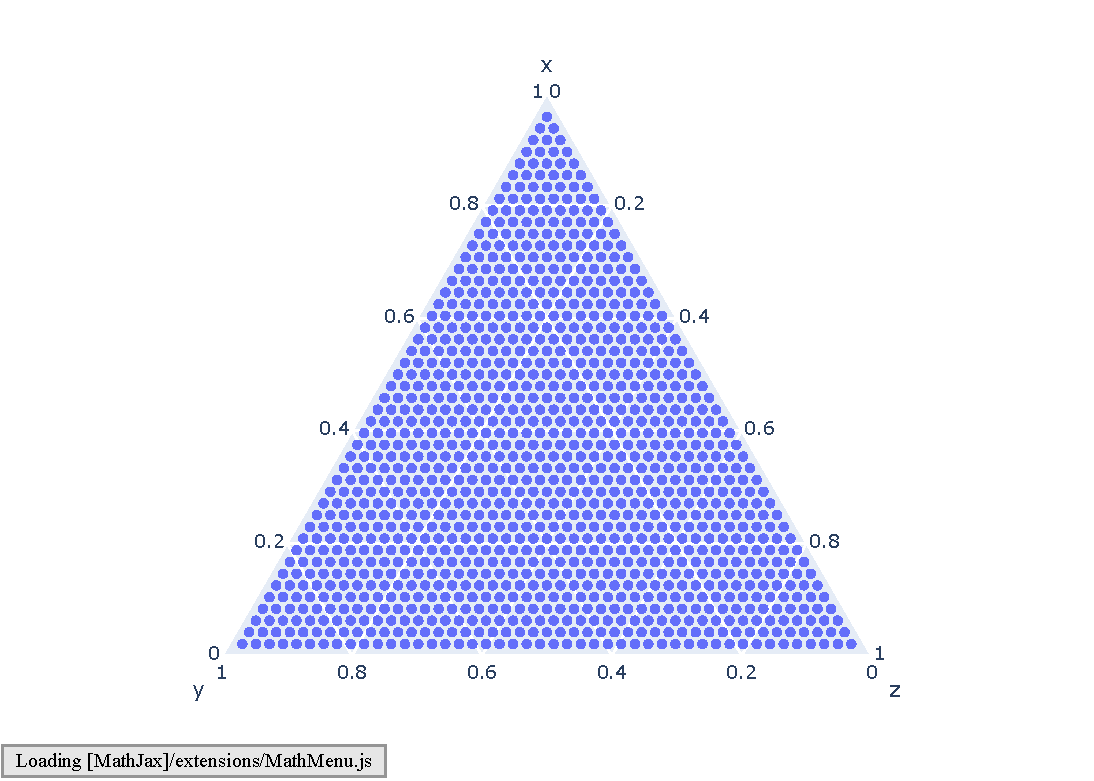
\includegraphics[width=0.55\textwidth]{nimplexTutorial1/01.QuickStart_17_0.pdf}
    \caption{A ternary full fractional simplex grid with $48$ divisions per dimension.}
    \label{nimplextutorial1:fig:ternarygrid}
\end{figure}

\textbf{Neat!}

You can also create a \textbf{uniform sampling} of the simplex space
using \texttt{simplex\_sampling\_mc}. Let us create a
\texttt{1000}-point sample of the simplex in
\texttt{3}-component space:

\begin{minted}[xleftmargin=3\parindent, linenos=true, fontsize=\small]{python}
randomSample1 = nimplex.simplex_sampling_mc_py(3, 2000)
randomSample1[:10]
\end{minted}

\begin{minted}[xleftmargin=3\parindent, fontsize=\small, bgcolor=subtlegray]{output}
[[0.5298803624052214, 0.07086239625884846, 0.3992572413359302],
 [0.0031033677260338954, 0.2388051480096958, 0.7580914842642703],
 [0.18649108765063374, 0.5836686212515504, 0.22984029109781595],
 [0.15016940727387892, 0.2949275122194682, 0.5549030805066528],
 [0.6155094564276237, 0.008656565578592935, 0.3758339779937834],
 [0.5304668735927556, 0.31073677219088075, 0.15879635421636376],
 [0.6207714545708731, 0.32969096943581894, 0.049537575993307915],
 [0.31938546746902047, 0.2709402919340315, 0.4096742405969479],
 [0.5712362080270665, 0.22399413177992233, 0.20476966019301104],
 [0.020101994689313802, 0.019307919101951364, 0.9605900862087349]]
\end{minted}

and plot it in 2D, just like before with the grid:

\begin{minted}[xleftmargin=3\parindent, linenos=true, fontsize=\small]{python}
randomSample1df = pd.DataFrame(randomSample1, columns=['x','y','z'])
px.scatter_ternary(randomSample1df, a='x', b='y', c='z', opacity=0.33)
\end{minted}

\begin{figure}[H]
    \centering
    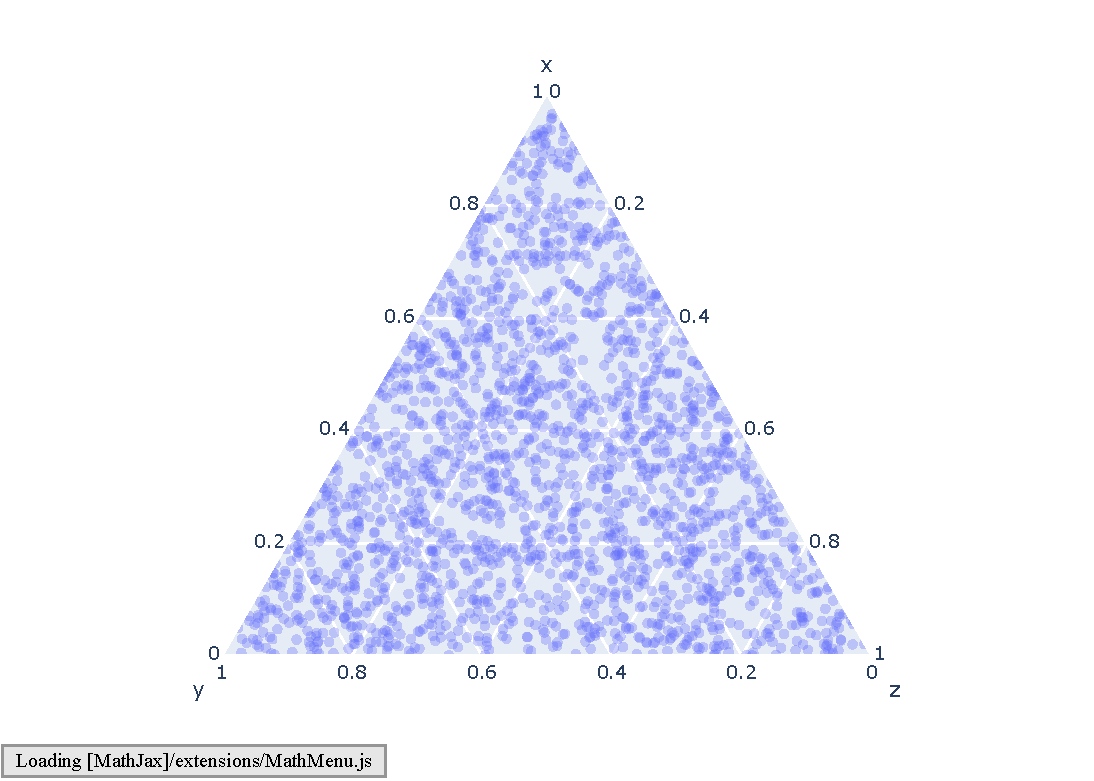
\includegraphics[width=0.55\textwidth]{nimplexTutorial1/01.QuickStart_22_0.pdf}
    \caption{A ternary uniform sampling of a simplex with $1000$ points.}
    \label{nimplextutorial1:fig:ternaryuniformsampling}
\end{figure}

The above works great for ternary (3-component) space, but what if we
want to work in quaternary (4-component) space which
\texttt{plotly} does not support directly? Or we want
to use a different plotting library without function like
\texttt{scatter\_ternary}? We can do so by projecting
the simplex onto the Euclidean space using the
\texttt{utils/plotting.nim} convenience module, which
was compiled as \texttt{plotting.so} and placed in the
\texttt{utils} in the current working directory. Let's
try it out:

\begin{minted}[xleftmargin=3\parindent, linenos=true, fontsize=\small]{python}
from utils import plotting
\end{minted}

\begin{minted}[xleftmargin=3\parindent, linenos=true, fontsize=\small]{python}
grid5_projected = plotting.simplex2cartesian_py(
  nimplex.simplex_internal_grid_fractional_py(3,48))
grid5_projected[:10]
\end{minted}

\begin{minted}[xleftmargin=3\parindent, fontsize=\small, bgcolor=subtlegray]{output}
[[-0.8118984375000001, -0.46875],
 [-0.7758140625000001, -0.46875],
 [-0.7397296875, -0.46875],
 [-0.7036453125000001, -0.46875],
 [-0.6675609375, -0.46875],
 [-0.6314765625, -0.46875],
 [-0.5953921875000001, -0.46875],
 [-0.5593078125000001, -0.46875],
 [-0.5232234375, -0.46875],
 [-0.48713906250000005, -0.46875]]
\end{minted}

As you can immediately notice, all points are now 2D vectors and now we
can plot the same grid as before, but using typical scatter plot
functionality:

\begin{minted}[xleftmargin=3\parindent, linenos=true, fontsize=\small]{python}
grid5_projected_df = pd.DataFrame(grid5_projected, columns=['x','y'])
px.scatter(grid5_projected_df, x='x', y='y', 
  width=600, height=500, template='plotly_white')
\end{minted}

\begin{figure}[H]
    \centering
    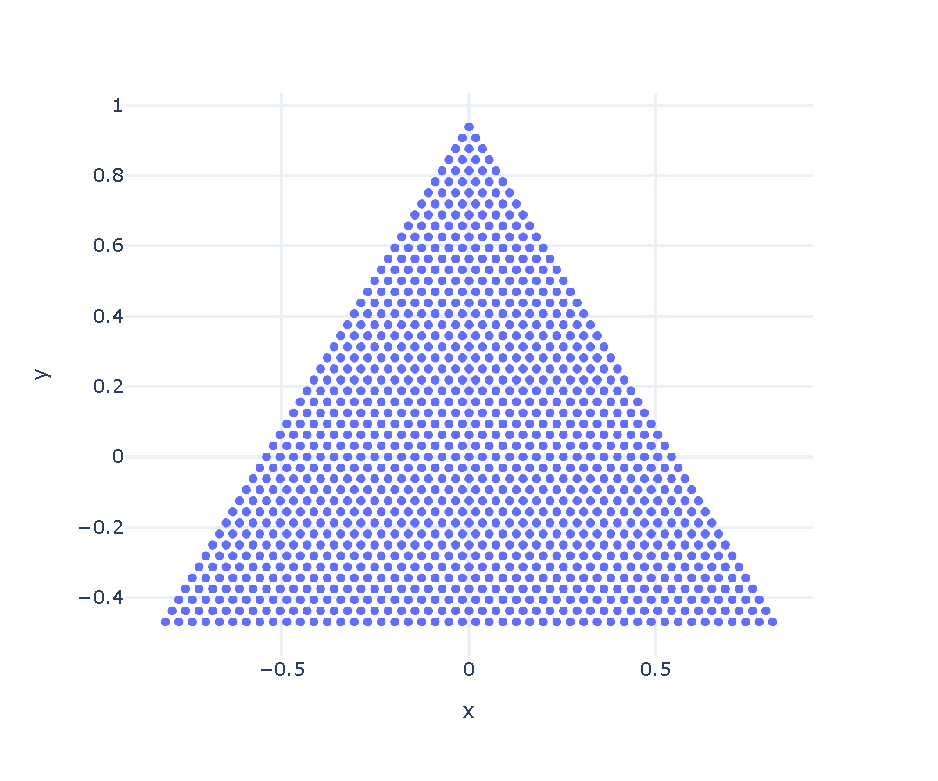
\includegraphics[width=0.55\textwidth]{nimplexTutorial1/01.QuickStart_27_0.pdf}
    \caption{A Cartesian space projection of ternary simplex grid through \texttt{nimplex}'s \texttt{utils.plotting.} \texttt{simplex2cartesian} function enabling plotting of Figure \ref{nimplextutorial1:fig:ternarygrid} in any 2D plotting software.}
    \label{nimplextutorial1:fig:ternarygridprojected}
\end{figure}

and then do the same for 4-component simplex space in 3D cartesian
space:

\begin{minted}[xleftmargin=3\parindent, linenos=true, fontsize=\small]{python}
grid6 = nimplex.simplex_internal_grid_fractional_py(4,12)
grid6_projected = plotting.simplex2cartesian_py(grid6)
grid6_projected[:10]
\end{minted}

\begin{minted}[xleftmargin=3\parindent, fontsize=\small, bgcolor=subtlegray]{output}
[[2.1806839667348754e-18, -8.4887374907083305e-19, 0.66666665],
 [-0.03928370999999999, -0.06804138333333333, 0.5555555333333333],
 [-0.07856742, -0.1360827666666667, 0.4444444166666667],
 [-0.11785112999999998, -0.20412415, 0.3333333],
 [-0.15713484, -0.2721655333333334, 0.22222218333333335],
 [-0.19641855, -0.3402069166666667, 0.11111106666666665],
 [-0.23570226000000002, -0.40824830000000006, -5.000000002919336e-08],
 [-0.27498596999999997, -0.4762896833333333, -0.11111116666666668],
 [-0.31426968, -0.5443310666666666, -0.22222228333333333],
 [-0.03928370999999999, 0.06804138333333333, 0.5555555333333333]]
\end{minted}

\begin{minted}[xleftmargin=3\parindent, linenos=true, fontsize=\small]{python}
grid6_projected_df = pd.DataFrame(grid6_projected, columns=['x','y','z'])
px.scatter_3d(grid6_projected_df, x='x', y='y', z='z', 
              template='plotly_white', width=800, height=700)
\end{minted}

\begin{figure}[H]
    \centering
    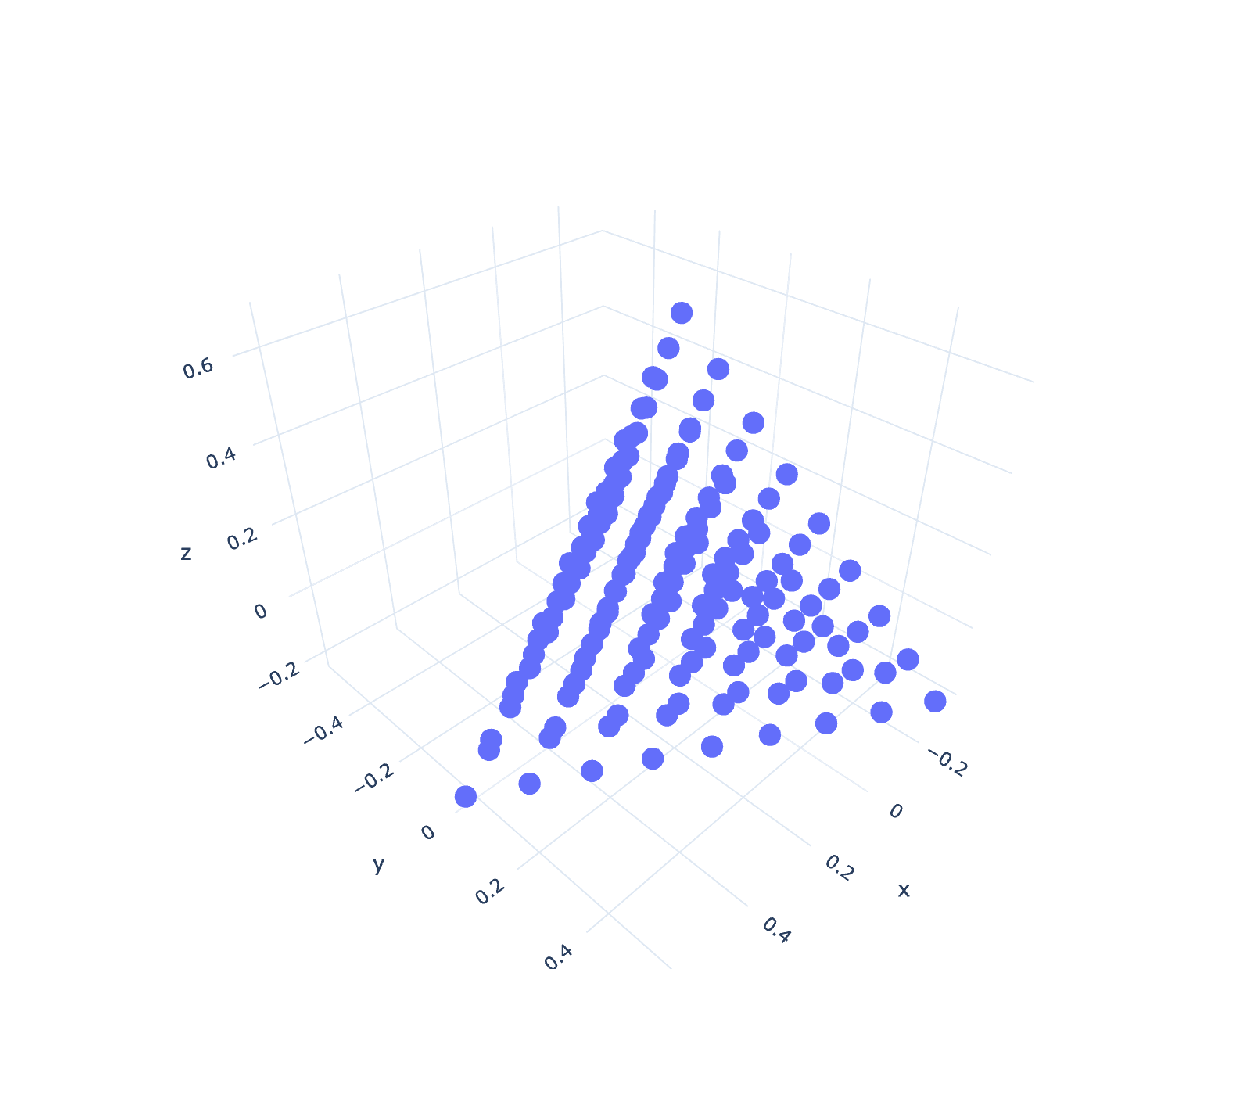
\includegraphics[width=0.6\textwidth]{nimplexTutorial1/01.QuickStart_30_0.pdf}
    \caption{A Cartesian space projection of quaternary simplex grid through \texttt{simplex2cartesian} enabling plotting in any 3D-capable software.}
    \label{nimplextutorial1:fig:quaternarygridprojected}
\end{figure}


or for random sampling:

\begin{minted}[xleftmargin=3\parindent, linenos=true, fontsize=\small]{python}
randomSample2 = plotting.simplex2cartesian_py(
  nimplex.simplex_sampling_mc_py(4, 1000))
randomSample2[:10]
\end{minted}

\begin{minted}[xleftmargin=3\parindent, fontsize=\small, bgcolor=subtlegray]{output}
[[-0.07501012159885143, 0.023590567429365657, -0.23553634907424525],
 [-0.4462490471332081, -0.1756565137829428, -0.2723228511523328],
 [0.07145506465222057, 0.3210603889969648, -0.18732905907855993],
 [-0.18725987909196115, 0.10689040149288015, -0.013098816843650607],
 [0.022355997592579786, 0.010927841672716905, -0.22642456944252606],
 [-0.0432501395787877, -0.17053829898879963, 0.11683087219672761],
 [0.037379243987826286, -0.050016213978314135, -0.031028495845089377],
 [0.01486956568331414, -0.0033756497464057025, 0.9054507810078116],
 [-0.08877119931676818, 0.13681189954017764, 0.6760960009121882],
 [0.38224893038975954, -0.16794340072714056, -0.15924029851917898]]
\end{minted}

\begin{minted}[xleftmargin=3\parindent, linenos=true, fontsize=\small]{python}
randomSample2df = pd.DataFrame(randomSample2, columns=['x','y','z'])
px.scatter_3d(randomSample2df, x='x', y='y', z='z', 
              template='plotly_white', width=800, height=700, opacity=0.2)
\end{minted}

\begin{figure}[H]
    \centering
    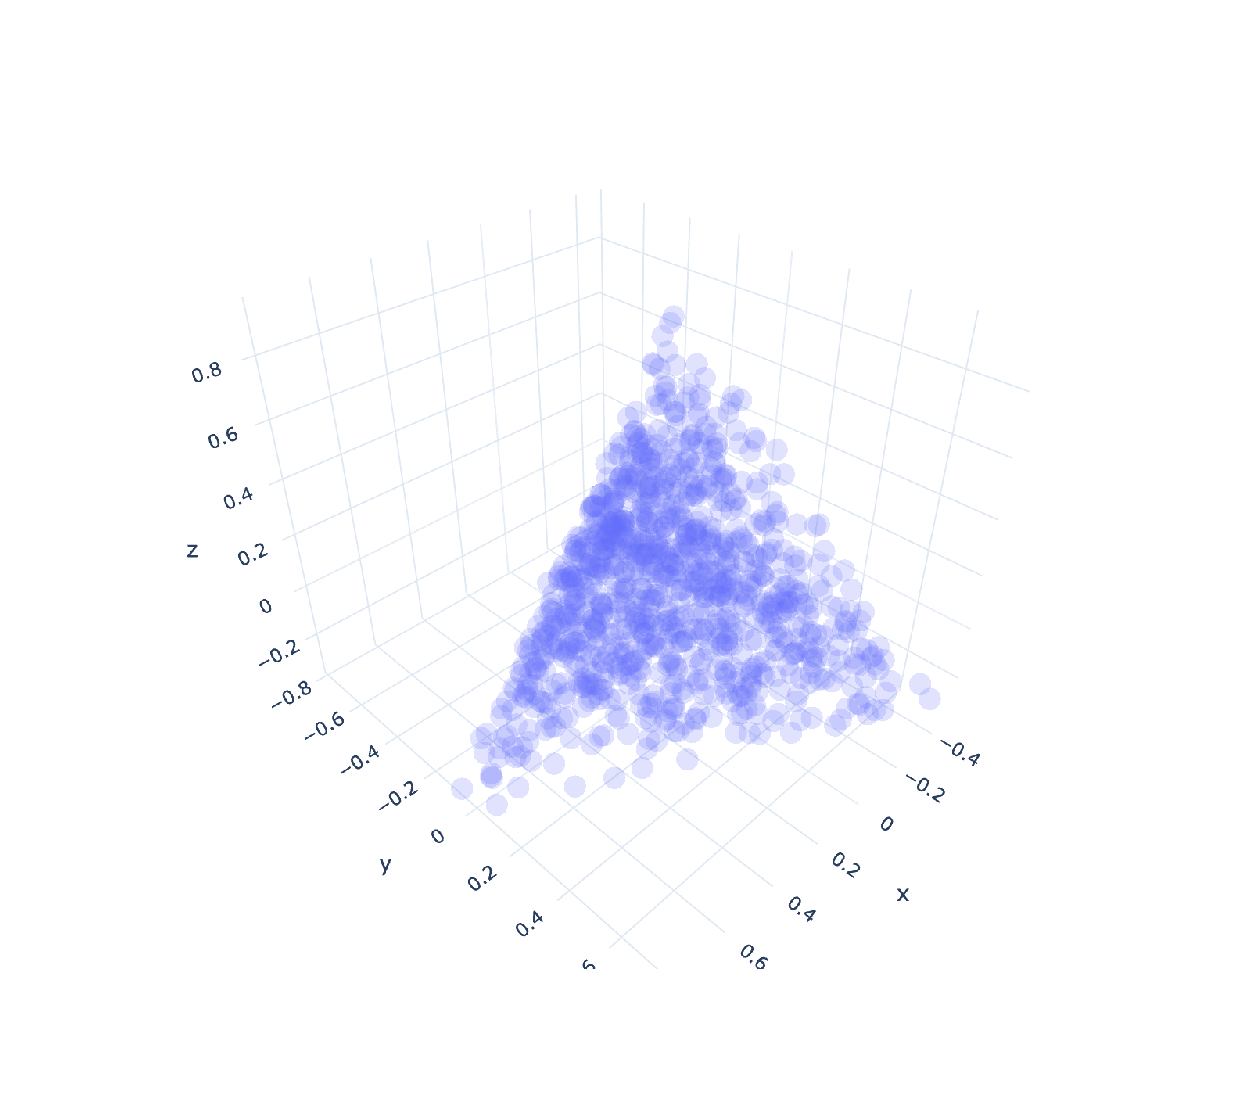
\includegraphics[width=0.6\textwidth]{nimplexTutorial1/01.QuickStart_33_0.pdf}
    \caption{A Cartesian space projection of quaternary simplex uniform sampling through \texttt{simplex2cartesian} enabling plotting in any 3D-capable software.}
    \label{nimplextutorial1:fig:quaternarysamlingprojected}
\end{figure}

Now, we can also attach \emph{some} model to it and see how it looks
like. Let's use Root Mean Squared Atomic Displacement (RMSAD) model for
high-entropy alloys (HEAs) in Ti-Zr-Hf-V-Nb-Ta-Mo-W-Re-Ru space designed
by Tandoc et al.~in
\href{https://doi.org/10.1038/s41524-023-00993-x}{10.1038/s41524-023-00993-x}
and reimplemented for \href{https://ultera.org}{ULTERA Ecosystem} by
nimplex's author. Let's now deploy it for a 4-component space formed by
\texttt{Ti}, \texttt{Zr},
\texttt{Hf}, and \texttt{V}, based on
\texttt{grid6} we generated before.

\begin{minted}[xleftmargin=3\parindent, linenos=true, fontsize=\small]{python}
import pqam_rmsadtandoc2023
\end{minted}

\begin{minted}[xleftmargin=3\parindent, linenos=true, fontsize=\small]{python}
components = ["Ti", "Zr", "Hf", "V"]
rmsadList = []
for point in grid6:
    formula = ' '.join([f'{c}{p}' for c, p in zip(components, point)])
    rmsadList.append(pqam_rmsadtandoc2023.predict(formula))
\end{minted}

\begin{minted}[xleftmargin=3\parindent, linenos=true, fontsize=\small]{python}
px.scatter_3d(grid6_projected_df, x='x', y='y', z='z', color=rmsadList,
              template='plotly_white', width=800, height=700)
\end{minted}

\begin{figure}[H]
    \centering
    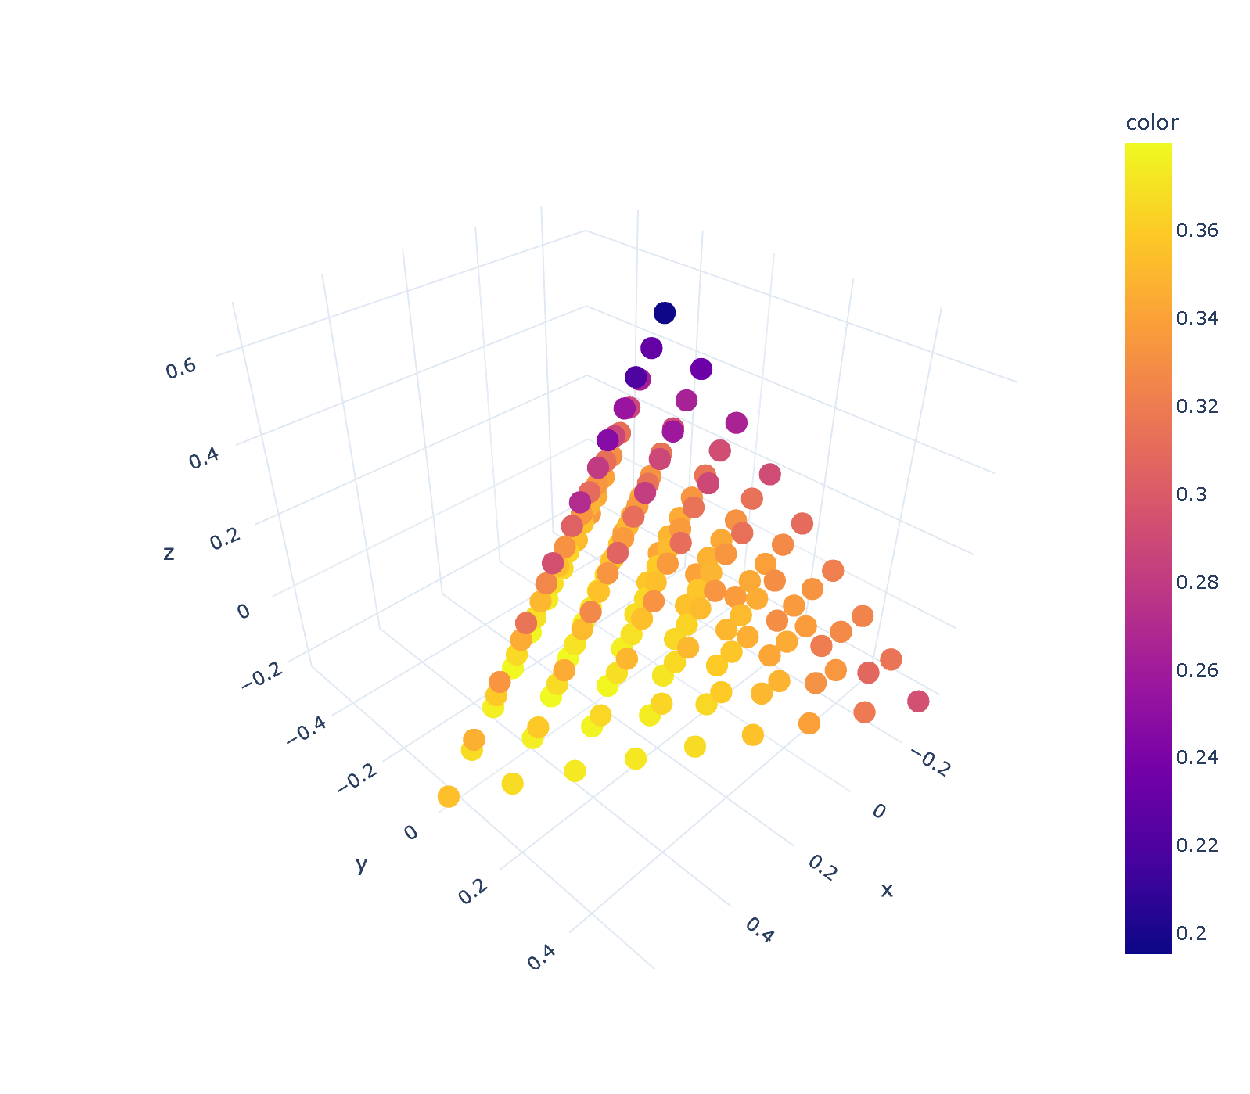
\includegraphics[width=0.6\textwidth]{nimplexTutorial1/01.QuickStart_37_0.pdf}
    \caption{Figure \ref{nimplextutorial1:fig:quaternarygridprojected} colorized by RMSAD predicted by model \cite{Tandoc2023MiningAlloys} deployed over Hf-Ti-V-Zr chemical space.}
    \label{nimplextutorial1:fig:quaternarygridcolored}
\end{figure}

But what if your system is not made of pure components, but rather of
some alloys? For that case you can generate a pair of \textbf{attainable
space} simplex grid and corresponding \textbf{elemental space} positions
serving as inputs to the model. Let's try it out for
\texttt{7}-component elemental space of
\texttt{Ti}, \texttt{Zr},
\texttt{Hf}, \texttt{W},
\texttt{Nb}, \texttt{Ta}, and
\texttt{Mo} formed by \texttt{4}
alloys: - Ti50 Zr50 - Hf95 Zr5 - Mo33 Nb33 Ta33 - Mo10 Nb10 W80

which we can represent as points in the elemental space:

\begin{minted}[xleftmargin=3\parindent, linenos=true, fontsize=\small]{python}
elementalSpaceComponents = 
  ["Ti", "Zr", "Hf", "W", "Nb", "Ta", "Mo"]
attainableSpaceComponents = 
  ["Ti50 Zr50", "Hf95 Zr5", "Mo33 Nb33 Ta33", "Mo10 Nb10 W80"]
attainableSpaceComponentPositions = 
  [[50, 50, 0, 0, 0, 0, 0], [0, 5, 95, 0, 0, 0, 0], 
  [0, 0, 0, 33, 33, 33, 0], [0, 0, 0, 10, 10, 0, 80]]
\end{minted}

and then generate the pair of grids:

\begin{minted}[xleftmargin=3\parindent, linenos=true, fontsize=\small, breaklines]{python}
gridAtt, gridEl = nimplex.embeddedpair_simplex_grid_fractional_py(attainableSpaceComponentPositions, 12)
\end{minted}

\begin{minted}[xleftmargin=3\parindent, linenos=true, fontsize=\small]{python}
gridAtt[:3]
\end{minted}

\begin{minted}[xleftmargin=3\parindent, fontsize=\small, bgcolor=subtlegray]{output}
[[0.0, 0.0, 0.0, 1.0],
 [0.0, 0.0, 0.08333333333333333, 0.9166666666666666],
 [0.0, 0.0, 0.16666666666666666, 0.8333333333333334]]
\end{minted}

\begin{minted}[xleftmargin=3\parindent, linenos=true, fontsize=\small]{python}
gridEl[:3]
\end{minted}

\begin{minted}[xleftmargin=3\parindent, fontsize=\small, bgcolor=subtlegray]{output}
[[0.0, 0.0, 0.0, 0.1, 0.1, 0.0, 0.8],
 [0.0,
  0.0,
  0.0,
  0.11944444444444445,
  0.11944444444444445,
  0.027777777777777776,
  0.7333333333333334],
 [0.0,
  0.0,
  0.0,
  0.1388888888888889,
  0.1388888888888889,
  0.05555555555555555,
  0.6666666666666667]]
\end{minted}

Then, we use the \textbf{elemental} space grid to run the model:

\begin{minted}[xleftmargin=3\parindent, linenos=true, fontsize=\small]{python}
rmsadList = []
for point in gridEl:
    formula = ' '.join([f'{c}{p}' for c, p in zip(elementalSpaceComponents, point)])
    rmsadList.append(pqam_rmsadtandoc2023.predict(formula))
\end{minted}

And \textbf{attainable} space grid to plot the results after projecting
them to the Euclidean space:

\begin{minted}[xleftmargin=3\parindent, linenos=true, fontsize=\small]{python}
gridAtt_projected_df = pd.DataFrame(
  plotting.simplex2cartesian_py(gridAtt), columns=['x','y','z'])
# Add text labels at the corners of the simplex
px.scatter_3d(gridAtt_projected_df, x='x', y='y', z='z', color=rmsadList,
              template='plotly_white', width=800, height=700, 
              labels={'color':'RMSAD', 'x':'', 'y':'', 'z':''})
\end{minted}

\begin{figure}[H]
    \centering
    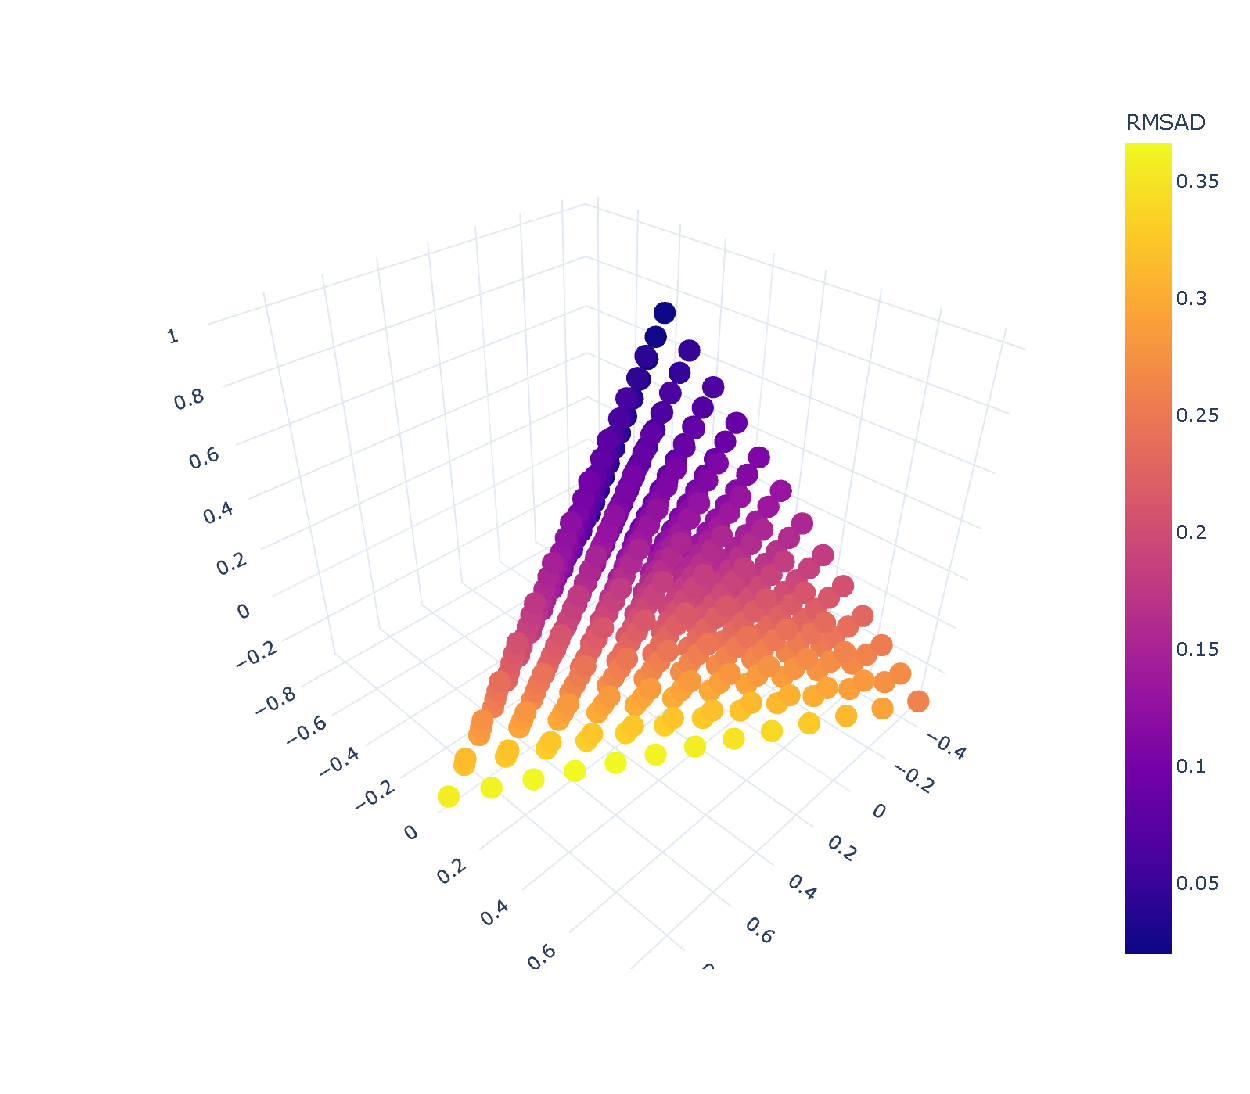
\includegraphics[width=0.6\textwidth]{nimplexTutorial1/01.QuickStart_47_0.pdf}
    \caption{Plot of RMSAD values over compositional tetrahedron (3-simplex) formed by all combinations of Ti50 Zr50, Hf95 Ti5, Mo33 Nb33 Ta33, Mo80 Nb10 W10 discretized at 12 divisions per dimension. The positions in the 7-component elemental space obtained from \texttt{nimplex} \cite{Krajewski2024Nimplex} were used to run RMSAD model by \cite{Tandoc2023MiningAlloys} and projected into Cartesian space for plotting by \texttt{simplex2cartesian} function in \texttt{nimplex}.}
    \label{nimplextutorial1:fig:quaternaryattainablecolored}
\end{figure}


we may also want to label the corners of the simplex with the alloy
names. We can do that by finding the indexes of the corners in the grid
using nimplex

\begin{minted}[xleftmargin=3\parindent, linenos=true, fontsize=\small]{python}
pureComponentIndices = nimplex.pure_component_indexes_py(4, 12)
print(pureComponentIndices)
\end{minted}

\begin{minted}[xleftmargin=3\parindent, fontsize=\small, bgcolor=subtlegray]{output}
[454, 90, 12, 0]
\end{minted}

\begin{minted}[xleftmargin=3\parindent, linenos=true, fontsize=\small]{python}
labels = ['']*len(gridAtt_projected_df)
for comp, idx in zip(attainableSpaceComponents, pureComponentIndices):
    labels[idx] = "<b>"+comp+"</b>"
\end{minted}

\begin{minted}[xleftmargin=3\parindent, linenos=true, fontsize=\small]{python}
gridAtt_projected_df = pd.DataFrame(
  plotting.simplex2cartesian_py(gridAtt), columns=['x','y','z'])
# Add text labels at the corners of the simplex
px.scatter_3d(gridAtt_projected_df, x='x', y='y', z='z', color=rmsadList, text=labels,
              template='plotly_white', width=800, height=700, 
              labels={'color':'RMSAD', 'x':'', 'y':'', 'z':''})
\end{minted}

\begin{figure}[H]
    \centering
    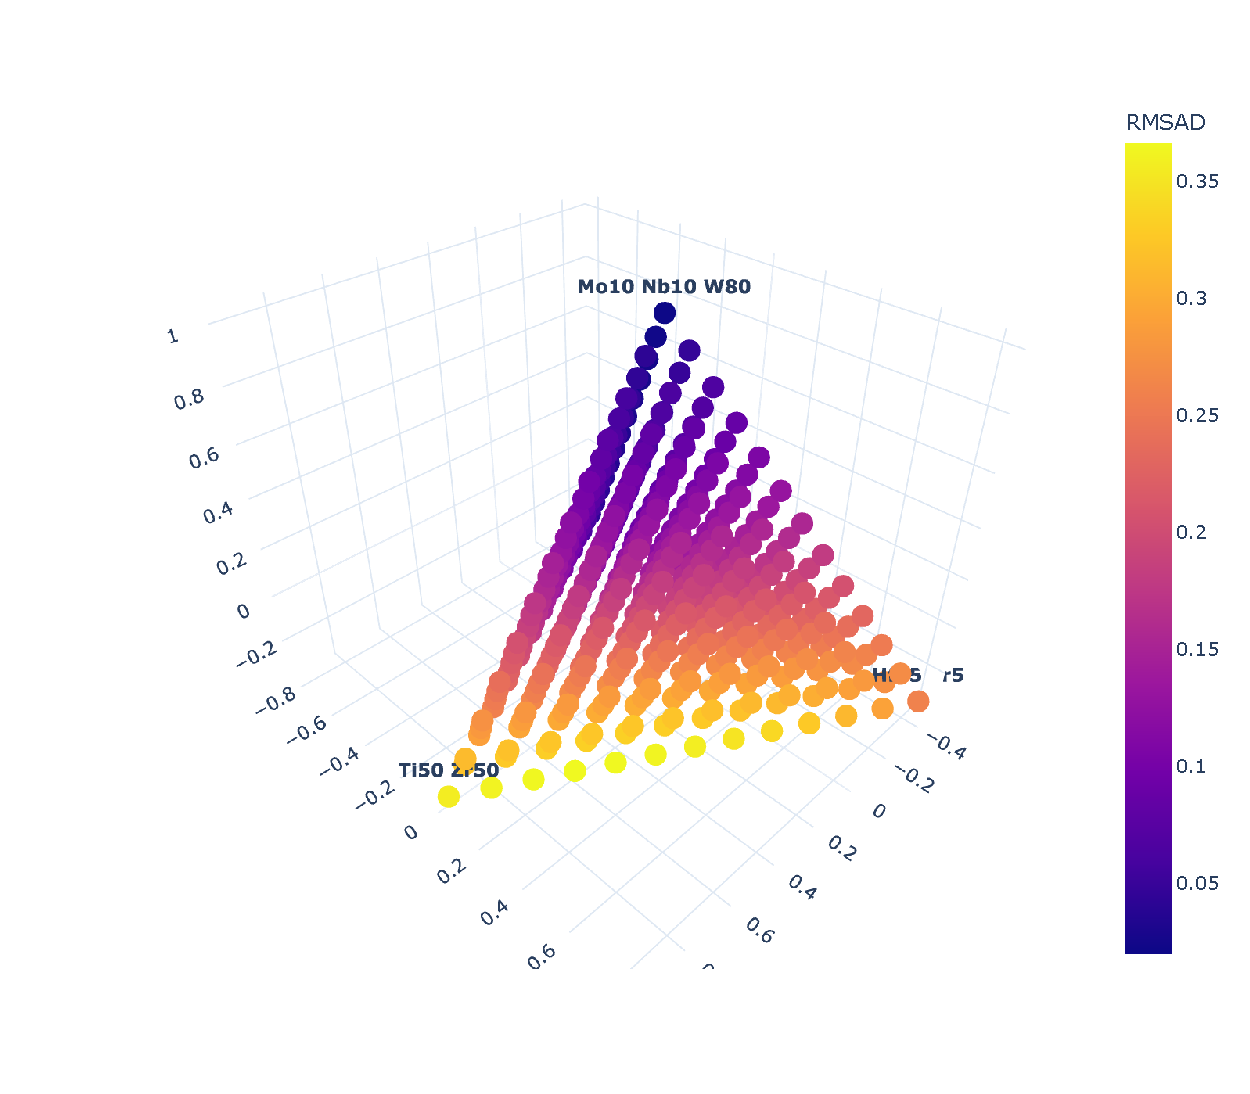
\includegraphics[width=0.6\textwidth]{nimplexTutorial1/01.QuickStart_51_0.pdf}
    \caption{Figure \ref{nimplextutorial1:fig:quaternaryattainablecolored} overlaid with pure-design-component (alloy composition) labels at spatial positions identified using \texttt{nimplex.pure\_component\_indexes}.}
    \label{nimplextutorial1:fig:quaternaryattainablecoloredlabel}
\end{figure}

\section{CLI - Grids and Random in Any Language from Julia to Ada
Samples} 
\label{nimplextutorial1:cli---grids-and-random-samples}

Let's say you don't want to use Python, but rather would like to use the
command line interface (CLI) to generate the grids and use them within,
e.g., \href{https://julialang.org}{Julia Language}. The easiest way to
do it is to output the grid to the common NumPy format, which you can
then then load it in Julia using one of the packages, such as
\href{https://www.juliapackages.com/p/npz}{NPZ.jl}.

The commands are concise, simple, and fully described in both
\href{https://amkrajewski.github.io/nimplex/}{documentation} and CLI
help:

\begin{minted}[xleftmargin=3\parindent, linenos=true, fontsize=\small]{python}
!./nimplex --help
\end{minted}

\begin{minted}[xleftmargin=3\parindent, fontsize=\small, bgcolor=subtlegray]{output}
To run nimplex please either (1) provide no arguments and follow the prompts or 
(2) use "-c" or "--config" to provide the configuration per instructions below:

- Provide the 3-letter configuration for task type:
    1. Grid type or uniform random sampling:
        - F: Full grid (including the simplex boundary)
        - I: Internal grid (only points inside the simplex)
        - R: Random/Monte Carlo uniform sampling over simplex.
        - G: Graph (list of grid nodes and list of their neighbors)
    2. Fractional or Integer positions:
        - F: Fractional grid/graph (points are normalized to fractions of 1)
        - I: Integer grid/graph (points are integers)
    3. Print full result, its shape, or persist in a file:
        - P: Print (presents full result as a table)
        - S: Shape (only the shape / size information)
        - N: Persist to NumPy array file ("nimplex_<configFlags>.npy" or 
             optionally a custom path as an additonal argument)

- Followed by integers of (1) simplex dimension and (2) number of divisions or
  samples depending on the task type. Optionally, custom output file path for 
  NumPy array can be provided as the last argument. E.g.:
    -c FFS [simplex dimension] [number of divisions]
    -c RFP [simplex dimension] [number of samples]
    -c FIN [simplex dimension] [number of divisions] [path/to/outfile.npy]

You can also utilize the following auxiliary flags:
--help       | -h   --> Show help.
--benchmark  | -b   --> Run benchmark for all tasks (9-dimensional space
                        with 12 divisions per dimension / 1M random samples).
\end{minted}

Based on the above, we can quickly generate a nice
\texttt{9}-component \texttt{I}nternal
simplex grid with \texttt{F}ractional with
\texttt{24} divisions per dimension and output it to
\texttt{N}numpy format file
\texttt{gridForJulia.npy}:

\begin{minted}[xleftmargin=3\parindent, linenos=true, fontsize=\small]{python}
!./nimplex --config IFN 9 24 gridForJulia.npy
\end{minted}

\begin{minted}[xleftmargin=3\parindent, fontsize=\small, bgcolor=subtlegray]{output}
Running with configuration:@["IFN", "9", "24", "gridForJulia.npy"]
Persisting to NumPy array file:gridForJulia.npy
Shape:[490314, 9]
\end{minted}

And wihinin a couple hundred miliseconds, we should get around 490,000
points of the grid neatly stored in the file of 36MB (on 64-bit system),
which we can now load it in Julia using

\begin{minted}[xleftmargin=3\parindent, fontsize=\small, bgcolor=subtlegray]{output}
using NPZ
data = npzread("gridForJulia.npy")
\end{minted}

In some cases, you may not have the ability to read the NumPy format,
because for instance, you are writing code for your favorite satellite
or train using a niche language like \href{https://ada-lang.io}{Ada}.
For situations like that, the backup option of formatter text output is
available. It is not nearly as efficient as the binary NumPy format, so
the grid from the last example would take minutes to generate, but it
should work with \emph{everything}.

Let's start by looking at a toy example. To get a small grid of
\texttt{3}-component \texttt{F}ull
simplex grid with \texttt{F}ractional with
\texttt{5} divisions per dimension, we can do:

\begin{minted}[xleftmargin=3\parindent, linenos=true, fontsize=\small]{python}
!./nimplex --config FFP 3 5
\end{minted}

\begin{minted}[xleftmargin=3\parindent, fontsize=\small, bgcolor=subtlegray]{output}
Running with configuration:@["FFP", "3", "5"]
Full Output:Tensor[system.float] of shape "[21, 3]" on backend "Cpu"
|0        0      1|
|0      0.2    0.8|
|0      0.4    0.6|
|0      0.6    0.4|
|0      0.8    0.2|
|0        1      0|
|0.2      0    0.8|
|0.2    0.2    0.6|
|0.2    0.4    0.4|
|0.2    0.6    0.2|
|0.2    0.8      0|
|0.4      0    0.6|
|0.4    0.2    0.4|
|0.4    0.4    0.2|
|0.4    0.6      0|
|0.6      0    0.4|
|0.6    0.2    0.2|
|0.6    0.4      0|
|0.8      0    0.2|
|0.8    0.2      0|
|1        0      0|
\end{minted}

As you can see, the first two lines of the output carry (1) task
metadata on what was run to create the grid, (2) output metadata
including its type(e.g.,
\texttt{int}/\texttt{float}/\texttt{float64}),
shape, and backend. Then the grid itself is printed out in the form of a
2D array with each row representing a single point and structured as
space-separated values between \texttt{|} characters.

To get a larger grid, we may want to stream the output to a file rather
than \texttt{P}rint it to the screen. We can do that by
redirecting the output to a file using \texttt{>}.
Let's create a \texttt{7}-component
\texttt{F}ull simplex grid with
\texttt{F}ractional with \texttt{12}
divisions per dimension and output it to
\texttt{gridForAda.txt}:

\begin{minted}[xleftmargin=3\parindent, linenos=true, fontsize=\small]{python}
!./nimplex --config FFP 7 12 > gridForAda.txt
\end{minted}

,which you can quickly read in Ada using rather elaborate code to parse
the file in strongly typed manner with some extra error checking. For
the sake of conciseness, it is not shown here, but the example below
shows how to do it in pure Python (using just built-in functions):

\begin{minted}[xleftmargin=3\parindent, linenos=true, fontsize=\small]{python}
with open('gridForAda.txt', 'r') as f:
    gridForAda = f.read()
    lines = gridForAda.replace('|', '').strip().split('\n')
    data = [[float(num) for num in line.split()] for line in lines[2:-1]]
\end{minted}

\begin{minted}[xleftmargin=3\parindent, linenos=true, fontsize=\small]{python}
data[:5]
\end{minted}

\begin{minted}[xleftmargin=3\parindent, fontsize=\small, bgcolor=subtlegray]{output}
[[0.0, 0.0, 0.0, 0.0, 0.0, 0.0, 1.0],
 [0.0, 0.0, 0.0, 0.0, 0.0, 0.0833333, 0.916667],
 [0.0, 0.0, 0.0, 0.0, 0.0, 0.166667, 0.833333],
 [0.0, 0.0, 0.0, 0.0, 0.0, 0.25, 0.75],
 [0.0, 0.0, 0.0, 0.0, 0.0, 0.333333, 0.666667]]
\end{minted}

\textbf{And now, you are ready to go and use nimplex in your favorite
language}

\textbf{In the second tutorial, in Appendix \ref{chap:nimplextutorial2} on 
Additive Manufacturing Path Planning, you will learn how to take advantage of the much more advanced graph construction functionality of nimplex to explore compositional spaces
and plan different traversal paths.}
